\documentclass[10.5pt]{beamer}
\usepackage[utf8]{inputenc}
\usetheme{PaloAlto}
%\usetheme{Madrid}
\usepackage[spanish]{babel}
\usepackage[T1]{fontenc}
\usepackage{amsmath}
\usepackage{amsfonts}
\usepackage{amssymb}
\usepackage{graphicx}
\usepackage{setspace}
\usepackage{ragged2e}
\usepackage{listings}
\usepackage{threeparttable}
\usepackage{array}
\title{Evaluadores y NURBS}
\author{Balboa Merly, Mirano Mitchell, Vasquez Sebastian}

\logo{
\includegraphics[scale=0.071]{figura/unmsm.png}}
\institute{UNMSM--Computación Cientfica}
 %\date{August 2022}
\date{\today}
%%%%%%%%%%%%%%%%%%%%%%%%%%%%%%%%%%%%%%%%%%%%%%%%%%%%%%%%%%%%%%%%%%%%%%%%%%%%%%%%%%%%%%%%%%%%%%
\begin{document}

\begin{frame}
\maketitle
\end{frame}


\begin{frame}{Contenido}
    %\small
    \tableofcontents
\end{frame}


\section{Introducción}

\begin{frame}{Introducción}
\begin{itemize}
\justifying
    \item  Las curvas y superficies suaves se dibujan aproximándolas con grandes o pequeños segmentos de línea o polígonos.
    \item   Muchas curvas y superficies pueden describirse matemáticamente mediante un pequeño número de parámetros.
    \item   Guardar 16 puntos de control para una superficie requiere menos almacenamiento que guardar 1000 triángulos junto con la información del vector normal en cada vértice. Además, sólo se aproximan a la superficie real, pero los puntos de control describen con precisión.
\end{itemize}
\end{frame}
%%%%%%%%%%%%%%%%%%%%%%%%%%%%%%%%%%%%%%%%%%%%%%%%%%%%%%%%%%%%%%%%%%%%%%%%%%%%%%%%%%%%%%%%%%%%%%%%%%
\begin{frame}{Introducción}
\begin{itemize}
\justifying
    \item  Si se quiere usar evaluadores para dibujar curvas y superficies utilizando otras bases, debemos convertir su base en una base de Bézier.
    \item   Cuando se renderiza una superficie Bézier o parte de ella utilizando evaluadores, es necesario especificar el nivel de detalle de su subdivisión.
\end{itemize}
\end{frame}
%%%%%%%%%%%%%%%%%%%%%%%%%%%%%%%%%%%%%%%%%%%%%%%%%%%%%%%%%%%%%%%%%%%%%%%%%%%%%%%%%%%%%%%%%%%%%%%%%%
\section{Evaluadores}

\begin{frame}{Evaluadores}
\begin{itemize}
\justifying
    \item Los evaluadores proporcionan una forma de especificar puntos en una curva o superficie utilizando puntos de control.
    \item   La curva o superficie puede ser renderizada con cualquier precisión. Además, los vectores normales pueden ser calculados automáticamente para las superficies.
    \item  Los puntos generados por un evaluador pueden utilizarse de muchas maneras: Para dibujar puntos donde estaría la superficie, una versión alámbrica de la superficie y una superficie completamente iluminada, sombreada e incluso texturizada.
\end{itemize}
\end{frame}

%%%%%%%%%%%%%%%%%%%%%%%%%%%%%%%%%%%%%%%%%%%%%%%%%%%%%%%%%%%%%%%%%%%%%%%%%%%%%%%%%%%%%%%%%%%%%%%%%%
\begin{frame}{Evaluadores}
\begin{itemize}
\justifying
    \item Se utilizan evaluadores para describir cualquier polinomio o splines polinómicos racionales o superficies de cualquier grado, incluye las B-splines, las NURBS (Non-Uniform Rational B-Spline), curvas y superficies Bézier y splines Hermite.

     \item   La función NURBS de la GLU es una interfaz de alto nivel: Los procesos NURBS encapsulan gran cantidad de código complejo. Gran parte del renderizado final se realiza con el evaluador, pero para ciertas condiciones (por ejemplo, recorte de curvas), los procesos NURBS utilizan polígonos planos para el renderizado.
\end{itemize}
\end{frame}
%%%%%%%%%%%%%%%%%%%%%%%%%%%%%%%%%%%%%%%%%%%%%%%%%%%%%%%%%%%%%%%%%%%%%%%%%%%%%%%%%%%%%%%%%%%%%%%%%%
\begin{frame}{Evaluadores}
\justifying
 Una curva de Bézier es una función vectorial de una variable
 \begin{block}
 \small
      \begin{equation*}
         C\left(u\right)=[X\left(u\right)Y\left(u\right)Z\left(u\right)]
      \end{equation*}
 \end{block}

Donde $u$ varía en un dominio $[0,1]$. Una superficie de Bézier es una función vectorial de dos variables.

El rango puede tener una salida tridimensional, bidimensional para curvas en un plano o coordenadas de textura,o una salida cuatridimensional para especificar información RGBA.
\end{frame}
%%%%%%%%%%%%%%%%%%%%%%%%%%%%%%%%%%%%%%%%%%%%%%%%%%%%%%%%%%%%%%%%%%%%%%%%%%%%%%%%%%%%%%%%%%%%%%%%%%
\begin{frame}{Evaluadores}
\begin{block}
\justifying
    Para utilizar un evaluador, primero hay que definir la función \textbf{C()} o \textbf{S()}, habilitarla y luego utilizar el comando \textbf{glEvalCoord1()} o \textbf{glEvalCoord2()} en lugar de \textbf{glVertex*()}.
\end{block}

\begin{itemize}
\justifying

    \item Los vértices de la curva o de la superficie pueden utilizarse como cualquier otro vértice, para formar puntos o líneas. Además, otros comandos generan automáticamente series de vértices que producen una malla regular uniformemente espaciada en u (o en u y v).
\end{itemize}
\end{frame}
%%%%%%%%%%%%%%%%%%%%%%%%%%%%%%%%%%%%%%%%%%%%%%%%%%%%%%%%%%%%%%%%%%%%%%%%%%%%%%%%%%%%%%%%%%%%%%%%%%
\subsection{Evaluadores unidimensionales}

\begin{frame}{Evaluadores unidimensionales}

\begin{figure}[h]
	\centering
	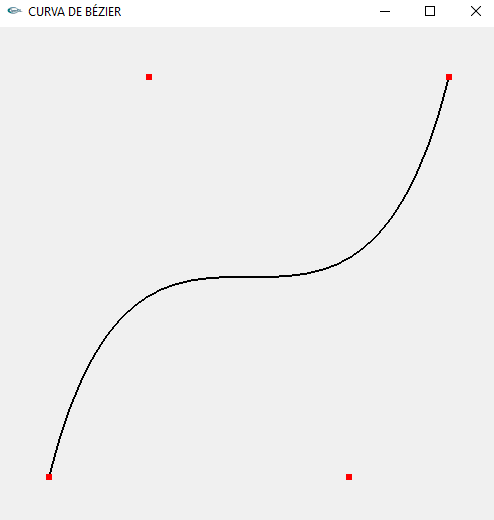
\includegraphics[width=0.5\linewidth]{figura/CURVA.PNG}
	\caption{Curva de Bézier.}
	\label{fig:propuesta}
\end{figure}

\end{frame}
%%%%%%%%%%%%%%%%%%%%%%%%%%%%%%%%%%%%%%%%%%%%%%%%%%%%%%%%%%%%%%%%%%%%%%%%%%%%%%%%%%%%%%%%%%%%%%%%%%
\subsection{Ejemplo}
\begin{frame}[fragile]
\justifying
\frametitle{Código}
La curva cúbica de Bézier se describe mediante cuatro puntos de control.
\begin{alertblock}{}
\small
\begin{verbatim}
GLfloat ctrlpoints[4][3] =
            {{-4.0, -4.0, 0.0}, { -2.0, 4.0, 0.0},
            {2.0, -4.0, 0.0}, {4.0, 4.0, 0.0}};
void init(void){
       glClearColor(0.94, 0.94, 0.94, 0.0);
       glShadeModel(GL_FLAT);
       glMap1f(GL_MAP1_VERTEX_3, 0.0, 1.0, 3, 4,
                            &ctrlpoints[0][0]);
       glEnable(GL_MAP1_VERTEX_3);
 }
\end{verbatim}
\end{alertblock}
La matriz \textbf{ctrlpoints[][]} es uno de los argumentos de \textbf{glMap1f()} y \textbf{glEnable()} habilita el evaluador unidimensional para vértices tridimensionales.
\end{frame}
%%%%%%%%%%%%%%%%%%%%%%%%%%%%%%%%%%%%%%%%%%%%%%%%%%%%%%%%%%%%%%%%%%%%%%%%%%%%%%%%%%%%%%%%%%%%%%%%%%
\begin{frame}[fragile]
\frametitle{Código}
La curva se dibuja en la rutina \textbf{display()} entre las llamadas \textbf{glBegin()} y \textbf{glEnd()}.

\begin{alertblock}{}
\small
\begin{verbatim}
    glColor3f(0.0, 0.0, 0.0);
    glBegin(GL_LINE_STRIP);
       for (int i = 0; i <= 30; i++)
           glEvalCoord1f((GLfloat) i/30.0);
    glEnd();
    glPointSize(6.0);
    glColor3f(1.0, 0.0, 0.0);
    glBegin(GL_POINTS);
        for (int i = 0; i < 4; i++)
           glVertex3fv(&ctrlpoints[i][0]);
    glEnd();
\end{verbatim}
\end{alertblock}
El comando \textbf{glEvalCoord1f()} es como emitir un \textbf{glVertex()} con las coordenadas de un vértice de la curva correspondiente al parámetro de entrada $u$.
\end{frame}
%%%%%%%%%%%%%%%%%%%%%%%%%%%%%%%%%%%%%%%%%%%%%%%%%%%%%%%%%%%%%%%%%%%%%%%%%%%%%%%%%%%%%%%%%%%%%%%%%%
\subsection{Definición y evaluación de un evaluador unidimensional}

\begin{frame}{Definición y evaluación de un evaluador unidimensional}
\justifying

El polinomio de Bernstein de grado n (u orden $n+1$ ) es dado por:
\begin{block}
\small
    \begin{equation*}
    B_i^n\left(u\right)=\left(\begin{matrix}n\\i\\\end{matrix}\right)u^i\left(1-u\right)^{n-i}
    \end{equation*}
\end{block}
Si $Pi$ representa un conjunto de puntos de control (unidimensionales, bidimensionales, tridimensionales o cuatridimensionales), entonces la ecuación:
\begin{block}
\small
    \begin{equation*}
   C\left(u\right)=\sum_{i=0}^{n}{B_i^n\left(u\right)}P_i
    \end{equation*}
\end{block}
Donde $B_{i}^{n}(u)$ son elementos de la distribución binomial respecto a $u$ y los $P_{i}$ son valores de la función que queremos aproximar.
\end{frame}
%%%%%%%%%%%%%%%%%%%%%%%%%%%%%%%%%%%%%%%%%%%%%%%%%%%%%%%%%%%%%%%%%%%%%%%%%%%%%%%%%%%%%%%%%%%%%%%%%%%%%
\begin{frame}{Definición y evaluación de un evaluador unidimensional}
\begin{itemize}
    \item Representa una curva de Bézier cuando $u$ varía de 0 a 1.
    \item Para representar la misma curva, pero permitiendo que, $u$ varíe entre $u1$ y $u2$ en lugar de 0 y 1, evaluamos:
    \begin{block}
     \small
    \begin{equation*}
          C\left(\frac{u-u_1}{u_2-u_1}\right)
    \end{equation*}
\end{block}
\end{itemize}
El comando \textbf{glMap1()} define un evaluador unidimensional que utiliza estas ecuaciones.\newline


\end{frame}

%%%%%%%%%%%%%%%%%%%%%%%%%%%%%%%%%%%%%%%%%%%%%%%%%%%%%%%%%%%%%%%%%%%%%%%%%%%%%%%%%%%%%%%%%%%%%%%%%%%%%
\begin{frame}{Definición y evaluación de un evaluador unidimensional}

   \begin{alertblock}{Comando}
   \small
    \textbf{glMap1\{fd\}} (GLenum target, TYPE u1, TYPE u2, GLint stride,
     GLint order, const TYPE *points);
   \end{alertblock}

   \begin{itemize}
   \justifying
       \item \textbf{GLenum target:} Especifica lo que representan los puntos de control, por lo tanto cuántos valores deben ser suministrados en puntos. Los puntos pueden representar vértices, datos de color RGBA, vectores normales o coordenadas de textura.

       \item \textbf{TYPE u1 y TYPE u2:} u1 y u2, indican el rango de la variable u.

       \item \textbf{GLint stride:} Es el número de valores de precisión simple o doble (según el caso) en cada bloque de almacenamiento. Por lo tanto, es un valor de desplazamiento entre el comienzo de un punto de control y el comienzo del siguiente.
   \end{itemize}

\end{frame}
%%%%%%%%%%%%%%%%%%%%%%%%%%%%%%%%%%%%%%%%%%%%%%%%%%%%%%%%%%%%%%%%%%%%%%%%%%%%%%%%%%%%%%%%%%%%%%%%%%%%%
\begin{frame}{Definición y evaluación de un evaluador unidimensional}

   \begin{alertblock}{Comando}
   \small
    \textbf{glMap1\{fd\}} (GLenum target, TYPE u1, TYPE u2, GLint stride,
     GLint order, const TYPE *points);
   \end{alertblock}

   \begin{itemize}
     \justifying
       \item \textbf{ GLint order:} El orden es el grado más uno, y debe coincidir con el número de puntos de control.

       \item \textbf{ const TYPE *points:} Los puntos apuntan a la primera coordenada del primer punto de control.
   \end{itemize}
  Utilizando la estructura de datos de ejemplo para glMap1*(), utilice lo siguiente para los puntos:
    \begin{alertblock}{}
   \small
   \begin{equation*}
       (GLfloat *) (\&ctrlpoints[0].x)
   \end{equation*}
   \end{alertblock}
\end{frame}
%%%%%%%%%%%%%%%%%%%%%%%%%%%%%%%%%%%%%%%%%%%%%%%%%%%%%%%%%%%%%%%%%%%%%%%%%%%%%%%%%%%%%%%%%%%%%%%%%%%%%

\begin{frame}{Definición y evaluación de un evaluador unidimensional}
    \justifying
Se utilizan los valores de los parámetros listados en la Tabla 1 para activar cada evaluador definido antes de invocarlo.

\begin{figure}[h]
	\centering
	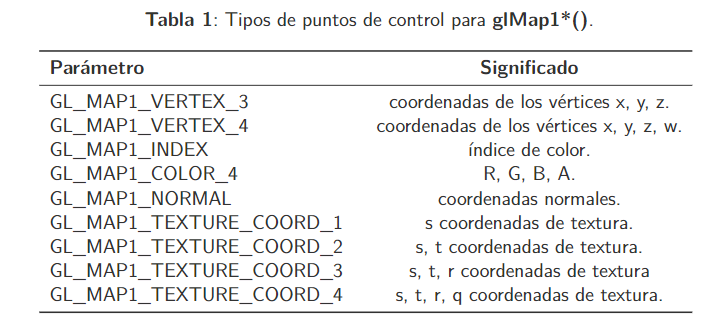
\includegraphics[width=1\linewidth]{figura/Tabla.PNG}
	%\caption{Curva de Bézier.}
	%\label{fig:propuesta}
\end{figure}
Pasamos el valor apropiado a \textbf{glEnable()} o \textbf{glDisable()} para activar o desactivar el evaluador.
\end{frame}

%%%%%%%%%%%%%%%%%%%%%%%%%%%%%%%%%%%%%%%%%%%%%%%%%%%%%%%%%%%%%%%%%%%%%%%%%%%%%%%%%%%%%%%%%%%%%%%%%%%%%
\begin{frame}[fragile]
    \frametitle{Definición y evaluación de un evaluador unidimensional}
    \justifying
\begin{itemize}
\justifying
    \item Se puede evaluar más de un evaluador a la vez. Si el evaluador GL\_MAP1\_VERTEX\_3 y  GL\_MAP1\_COLOR\_4 son definidos y habilitados, entonces \textbf{glEvalCoord1()} generan una posición como un color.

    \item Si se define y activa más de un evaluador del mismo tipo, se utiliza el de mayor dimensión.

    \item Utilizamos \textbf{glEvalCoord1*()} para evaluar un mapa unidimensional definido y habilitado.
\end{itemize}

\begin{alertblock}{}
\small
\begin{verbatim}
          void glEvalCoord1{fd} (TYPE u);
          void glEvalCoord1{fd} v (TYPE *u);
\end{verbatim}
\end{alertblock}

 Provoca la evaluación de mapas unidimensionales habilitados. El argumento $u$ es el valor (o un puntero al valor, en la versión vectorial del comando) de la coordenada del dominio.
\end{frame}
%%%%%%%%%%%%%%%%%%%%%%%%%%%%%%%%%%%%%%%%%%%%%%%%%%%%%%%%%%%%%%%%%%%%%%%%%%%%%%%%%%%%%%%%%%%%%%%%%%%%%
\subsection{Definición de valores de coordenadas uniformes en una dimensión}

\begin{frame}[fragile]
 \frametitle{Definición de valores de coordenadas uniformes en una dimensión}

\begin{itemize}
\justifying
    \item Se puede utilizar \textbf{glEvalCoord1()} con cualquier valor para $u$, pero el uso más común es con valores espaciados uniformemente, como se muestra en el Ejemplo 1.

    \item Para obtener valores uniformemente espaciados, definimos una unidimensional usando \textbf{glMapGrid1*()} y aplícamos usando \textbf{glEvalMesh1()}.
\end{itemize}

\begin{alertblock}{}
\small
\begin{verbatim}
    void glMapGrid1{fd} (GLint n, TYPE u1, TYPE u2);
\end{verbatim}
\end{alertblock}
Define una cuadrícula que va de $u1$ a $u2$ en $n$ pasos, que están espaciados uniformemente.
\begin{alertblock}{}
\small
\begin{verbatim}
    void glEvalMesh1(GLenum mode, GLint p1, GLint p2);
\end{verbatim}
\end{alertblock}
\end{frame}

%%%%%%%%%%%%%%%%%%%%%%%%%%%%%%%%%%%%%%%%%%%%%%%%%%%%%%%%%%%%%%%%%%%%%%%%%%%%%%%%%%%%%%%%%%%%%%%%%%%%%
\subsection{Definición de valores de coordenadas uniformes en una dimensión}

\begin{frame}[fragile]
 \frametitle{Definición de valores de coordenadas uniformes en una dimensión}

\begin{itemize}
\justifying
    \item Aplica la cuadrícula de mapa definida actualmente a todos los evaluadores habilitados. El modo puede ser \textbf{GL\_POINT o GL\_LINE}, dependiendo de si desea dibujar puntos o una línea conectada a lo largo de la curva.

    \item  Tiene exactamente el mismo efecto que emitir una \textbf{glEvalCoord1()} para cada uno de los pasos, incluyendo $p1$ y $p2$, donde $0\le\ p1,\ p2\le\ n$. Es equivalente a lo siguiente:
\end{itemize}

\begin{alertblock}{}
\small
\begin{verbatim}
  glBegin(GL_POINTS); /* o glBegin(GL_LINE_STRIP);*/
      for (i = p1; i <= p2; i++)
          glEvalCoord1(u1 + i*(u2-u1)/n);
  glEnd();
\end{verbatim}
\end{alertblock}
Excepto si \textbf{i = 0} o \textbf{i = n}, entonces se llama a \textbf{glEvalCoord1()} con exactamente $u1$ o $u2$ como parámetro.
\end{frame}
%%%%%%%%%%%%%%%%%%%%%%%%%%%%%%%%%%%%%%%%%%%%%%%%%%%%%%%%%%%%%%%%%%%%%%%%%%%%%%%%%%%%%%%%%%%%%%%%%%%%%

\subsection{Evaluadores bidimensionales}

\begin{frame}[fragile]
\frametitle{Evaluadores bidimensionales}

En dos dimensiones, todo es similar al caso unidimensional, excepto que todos los comandos deben
tener en cuenta dos parámetros, U y V,. Los puntos, colores, normales o coordenadas de textura deben ser
suministrado sobre una superficie en lugar de una curva. Matemáticamente, la definición de un parche de superficie Bézier es
dada por

\begin{block}

\begin{equation*}
    S(u,v)=\sum_{i=0}^{n}\sum_{j=0}^{m} B_{i}^{n}(u) B_{j}^{m}(v)P_{ij}
\end{equation*}

\end{block}

donde $P_{ij}$ son un conjunto de puntos de control $m*n$ y los $B_{i}$ son los mismos polinomios de Bernstein para uno
dimensión. Como antes, el $P_{ij}$ puede representar vértices, normales, colores o coordenadas de textura.
\end{frame}
%%%%%%%%%%%%%%%%%%%%%%%%%%%%%%%%%%%%%%%%%%%%%%%%%%%%%%%%%%%%%%%%%%%%%%%%%%%%%%%%%%%%%%%%%%%%%%%%%%%%%

\begin{frame}[fragile]
    \frametitle{Evaluadores bidimensionales}

El procedimiento para usar evaluadores bidimensionales es similar al procedimiento para una dimensión.

\begin{itemize}
    \item Defina los evaluadores(s) con glMap2*()
    \item Habilitarlos pasando el valor apropiado a glEnable().
    \item Invocarlos llamando a glEvalCoord2() entre un par glBegin() y glEnd() o por
    Especificar y luego aplicar una malla con glMapGrid2() y glEvalMesh2().
\end{itemize}


\end{frame}
%%%%%%%%%%%%%%%%%%%%%%%%%%%%%%%%%%%%%%%%%%%%%%%%%%%%%%%%%%%%%%%%%%%%%%%%%%%%%%%%%%%%%%%%%%%%%%%%%%%%%
\begin{frame}[fragile]
    \frametitle{Definición y evaluación de un evaluador bidimensional}

    Use GLMAP2*() y GlevalCoord2*() para definir y luego invocar un evaluador bidimensional.
    void glMap2{fd}(GLenum target, TYPEu1, TYPEu2, GLint ustride,
    GLint uorder, TYPEv1, TYPEv2, GLint vstride,
    GLint vorder, TYPE points);

    El parámetro objetivo puede tener cualquiera de los valores de la tabla, excepto que la cadena MAP1 es
    reemplazado con MAP2. Como antes, estos valores también se usan con glEnable() para habilitar el
    evaluador correspondiente. Los valores mínimos y máximos para U y V se proporcionan como U1, U2,
    V1 y V2. Los parámetros de ustride y vstride indican el número de precisión única o doble
    valores (según corresponda) entre la configuración independiente para estos valores,
    lo que permite a los usuarios seleccionar un
    el subrectangulo de control señalada en  una matriz mucho más grande.
    \begin{alertblock}{}
        \small
        \center
            GLfloat ctlpoints[100][100][3];
    \end{alertblock}
\end{frame}
%%%%%%%%%%%%%%%%%%%%%%%%%%%%%%%%%%%%%%%%%%%%%%%%%%%%%%%%%%%%%%%%%%%%%%%%%%%%%%%%%%%%%%%%%%%%%%%%%%%%%

\begin{frame}[fragile]
    \frametitle{Definición y evaluación de un evaluador bidimensional}
    y desea usar el subconjunto 4x4 que comienza en cltpoints[20][30], elija Ustride para que sea 100*3 y
    Vstride para ser 3. El punto de partida, puntos, debe establecerse en $\&ctlpoints[20][30][0]$. Finalmente,
    los parámetros de pedido, Uorder y Vorder pueden ser diferentes, lo que permite parches cúbicos en uno
    dirección y cuadrática en el otro, por ejemplo.

    \begin{itemize}
        \item void glEvalCoord2{fd}(TYPE u, TYPE v)
        \item void glEvalCoord2{fd}v(TYPE *values)
    \end{itemize}

\end{frame}
%%%%%%%%%%%%%%%%%%%%%%%%%%%%%%%%%%%%%%%%%%%%%%%%%%%%%%%%%%%%%%%%%%%%%%%%%%%%%%%%%%%%%%%%%%%%%%%%%%%%%

\begin{frame}[fragile]
     Los argumentos U y V son los valores(o un puntero a los valores U y V, en la versión vectorial del comando) para las coordenadas de dominio.
    Si se habilita cualquiera de los evaluadores de vértices ($ GL\_MAP2\_VERTEX\_3 $ o $ GL\_MAP2\_VERTEX\_4 $),
    entonces lo normal a la superficie se calcula analíticamente. Esta normal está asociada con el
    vértice generado si la generación normal automática se ha habilitado pasando
    $GL\_AUTO\_NORMAL$ a glEnable(). Si está deshabilitado, el mapa normal habilitado habilitado correspondiente es
    utilizado para producir una normal. Si no existe tal mapa, se usa la corriente actual.

    El siguiente(12-2) ejemplo dibuja una superficie de estructura bézier utilizando evaluadores, en este
    ejemplo, la superficie se dibuja con nueve líneas curvas en cada dirección. Cada curva se dibuja como 30
    segmentos.

\end{frame}
%%%%%%%%%%%%%%%%%%%%%%%%%%%%%%%%%%%%%%%%%%%%%%%%%%%%%%%%%%%%%%%%%%%%%%%%%%%%%%%%%%%%%%%%%%%%%%%%%%%%%

\subsection{Definición de valores de coordenadas espaciados uniformemente en dos dimensiones}

\begin{frame}[fragile]
\frametitle{Definición de valores de coordenadas espaciados uniformemente en dos dimensiones}

En dos dimensiones, los comandos glMapGrid2*() y glEvalMesh2() son similares a los
Versiones unidimensionales, excepto que se deben incluir información de U y V.

\begin{itemize}
    \item void glMapGrid2{fd}(GLint nu, TYPEu1, TYPEu2,
    GLint nv, TYPEv1, TYPEv2);
    \item void glEvalMesh2(GLenum mode, GLint i1, GLint i2, GLint j1, GLint j2);
\end{itemize}

Define una cuadrícula de mapa bidimensional que va de U1 a U2 en pasos nu uniformemente espaciados, de V1 a
V2 en pasos NV (glMapGrid2*()), y luego aplica esta cuadrícula a todos los evaluadores habilitados
(glEvalMesh2()).

\end{frame}
%%%%%%%%%%%%%%%%%%%%%%%%%%%%%%%%%%%%%%%%%%%%%%%%%%%%%%%%%%%%%%%%%%%%%%%%%%%%%%%%%%%%%%%%%%%%%%%%%%%%%

\begin{frame}[fragile]
    \frametitle{Definición de valores de coordenadas espaciados uniformemente en dos dimensiones}

La única diferencia significativa con las versiones unidimensionales de estos dos. Los comandos en glevalmesh2 () el parámetro de modo puede ser $GL\_FILL$ y $GL\_POINT$
o $GL\_LINE$ $GL\_FILL$ genera polígonos rellenos utilizando el primitivo de malla cuádruple. Declarado precisamente,
GlevalMesh2()

\begin{alertblock}{}
    \small
    \begin{verbatim}
    glBegin(GL_POINTS); /* mode == GL_POINT */
    for (i = nu1; i <= nu2; i++)
    for (j = nv1; j <= nv2; j++)
    glEvalCoord2(u1 + i*(u2-u1)/nu, v1+j*(v2-v1)/nv);
    glEnd();
    \end{verbatim}
\end{alertblock}
\end{frame}
%%%%%%%%%%%%%%%%%%%%%%%%%%%%%%%%%%%%%%%%%%%%%%%%%%%%%%%%%%%%%%%%%%%%%%%%%%%%%%%%%%%%%%%%%%%%%%%%%%%%%

\begin{frame}[fragile]
    \frametitle{Definición de valores de coordenadas espaciados uniformemente en dos dimensiones}

\begin{alertblock}{}
    \small
    \begin{verbatim}

    for (i = nu1; i <= nu2; i++) { /* mode == GL_LINE */
    glBegin(GL_LINES);
        for (j = nv1; j <= nv2; j++)
        glEvalCoord2(u1 + i*(u2-u1)/nu, v1+j*(v2-v1)/nv);
    glEnd();
    }

    for (j = nv1; j <= nv2; j++) {
    glBegin(GL_LINES);
        for (i = nu1; i <= nu2; i++)
        glEvalCoord2(u1 + i*(u2-u1)/nu, v1+j*(v2-v1)/nv);
    glEnd();
    }
    \end{verbatim}
\end{alertblock}
\end{frame}
%%%%%%%%%%%%%%%%%%%%%%%%%%%%%%%%%%%%%%%%%%%%%%%%%%%%%%%%%%%%%%%%%%%%%%%%%%%%%%%%%%%%%%%%%%%%%%%%%%%%%


\begin{frame}[fragile]
    \frametitle{Definición de valores de coordenadas espaciados uniformemente en dos dimensiones}

\begin{alertblock}{}
    \small
    \begin{verbatim}
    for (i = nu1; i < nu2; i++) { /* mode == GL_FILL */
    glBegin(GL_QUAD_STRIP);
    for (j = nv1; j <= nv2; j++) {
      glEvalCoord2(u1+i*(u2-u1)/nu,v1+j*(v2-v1)/nv);
      glEvalCoord2(u1+(i+1)*(u2-u1)/nu,v1+j*(v2-v1)/nv);
    glEnd();
        }
    }
\end{verbatim}
\end{alertblock}

El siguiente ejemplo(12-3) muestra las diferencias necesarias para dibujar la misma superficie de Bézier que el ejemplo 12-2, pero
Usando glMapGrid2() y glEvalMesh2() para subdividir el dominio cuadrado en una cuadrícula uniforme de 8x8.

\end{frame}
%%%%%%%%%%%%%%%%%%%%%%%%%%%%%%%%%%%%%%%%%%%%%%%%%%%%%%%%%%%%%%%%%%%%%%%%%%%%%%%%%%%%%%%%%%%%%%%%%%%%%

\subsection{Usar evaluadores para texturas}
\begin{frame}[fragile]
\frametitle{Usar evaluadores para texturas}
\small
En el siguiente ejemplo se  habilita dos evaluadores al mismo tiempo: el primero genera puntos tridimensionales en
la misma superficie de Bézier del ejemplo anterior, y la segunda genera coordenadas de textura. En este caso, el
Las coordenadas de textura son las mismas que las coordenadas U y V de la superficie, pero un parche especial de Bézier
debe crearse para hacer esto.
El parche plano se define sobre un cuadrado con esquinas en (0, 0), (0, 1), (1, 0) y (1, 1);genera (0, 0) en
esquina (0, 0), (0, 1) en la esquina (0, 1), y así sucesivamente. Ya que es de orden dos (grado lineal más uno), evaluando

Esta textura en el punto (U, V) genera coordenadas de textura (S, T). Está habilitado al mismo tiempo que el
Evaluador de vértice, por lo que ambos surtan efecto cuando se dibuja la superficie. Si
Desea que la textura repita tres veces en cada dirección, cambie cada 1.0 en la matriz texpts[][][] a 3.0.
Dado que la textura se envuelve en este ejemplo, la superficie se representa con nueve copias del mapa de textura.
\end{frame}

%%%%%%%%%%%%%%%%%%%%%%%%%%%%%%%%%%%%%%%%%%%%%%%%%%%%%%%%%%%%%%%%%%%%%%%%%%%%%%%%%%%%%%%%%%%%%%%%%%%%%

\section{Interfaz GLU NURBS}
\begin{frame}[fragile]
\frametitle{Interfaz GLU NURBS}
\small
\begin{itemize}
    \justifying
    \item Aunque los evaluadores son la única primitiva de OpenGL
    disponible para dibujar curvas y superficies directamente,
    y aunque se pueden implementar de manera muy eficiente en hardware,
    las aplicaciones a menudo acceden a ellos a través
    de bibliotecas de nivel superior.
    \item   GLU proporciona una interfaz NURBS (Non-Uniform Rational B-Spline)
    construida sobre los comandos del evaluador OpenGL.
    \item   Si entiende NURBS, escribir código OpenGL para
    manipular curvas y superficies NURBS es relativamente
    fácil, incluso con iluminación y mapeo de texturas.
\end{itemize}
\end{frame}

%%%%%%%%%%%%%%%%%%%%%%%%%%%%%%%%%%%%%%%%%%%%%%%%%%%%%%%%%%%%%%%%%%%%%%%%%%%%%%%%%%%%%%%%%%%%%%%%%%%%%

\begin{frame}[fragile]
\frametitle{Ejemplo simple de NURBS}
\small
Pasos para dibujar curvas NURBS o superficies NURBS sin recortar.
\begin{itemize}
    \item[1.] \textbf{glEnable()} con GL\_AUTO\_NORMAL para generar superficies normales.
    \item[2.] Utilice \textbf{gluNewNurbsRenderer()} para crear un puntero
    a un objeto NURBS.
    \item[3.] \textbf{gluNurbsProperty()} para valores de representación,
    como el tamaño máximo de líneas o polígonos.
    \item[4.] Llame a \textbf{gluNurbsCallback()} si desea que se le notifique
    cuando se encuentre un error.
    \item[5.] Inicie su curva o superficie llamando a \textbf{gluBeginCurve()}
    o \textbf{gluBeginSurface()}.
    \item[6.] Genera y renderiza tu curva o superficie \textbf{gluNurbsCurve()} o \textbf{gluNurbsSurface()}
    \item[7.] \textbf{gluEndCurve()} o \textbf{gluEndSurface()}
    para completar la curva o superficie.
\end{itemize}
\end{frame}

%%%%%%%%%%%%%%%%%%%%%%%%%%%%%%%%%%%%%%%%%%%%%%%%%%%%%%%%%%%%%%%%%%%%%%%%%%%%%%%%%%%%%%%%%%%%%%%%%%%%%

\begin{frame}[fragile]
\frametitle{Administrar objetos NURBS}
\small

\begin{alertblock}{Comando}
    \small
    \emph{GLUnurbsObj* \textbf{gluNewNurbsRenderer}(void);}
\end{alertblock}

\begin{itemize}
    \justifying
    \item Crea un nuevo objeto NURBS, nobj.
    Devuelve un puntero al nuevo objeto, o cero, si OpenGL no
    puede asignar memoria para un nuevo objeto NURBS.
\end{itemize}

\begin{alertblock}{Comando}
    \small
    \emph{void \textbf{gluDeleteNurbsRenderer}(GLUnurbsObj *nobj);}
\end{alertblock}

\begin{itemize}
    \justifying
    \item Destruye el objeto NURBS nobj.
\end{itemize}

\end{frame}

%%%%%%%%%%%%%%%%%%%%%%%%%%%%%%%%%%%%%%%%%%%%%%%%%%%%%%%%%%%%%%%%%%%%%%%%%%%%%%%%%%%%%%%%%%%%%%%%%%%%%

\begin{frame}[fragile]
\frametitle{Control de propiedades de renderización de NURBS}
\small

Un conjunto de propiedades asociadas con un objeto NURBS afecta la
forma en que el objeto es renderizado. Estas propiedades incluyen
cómo se rasteriza la superficie (por ejemplo, relleno o estructura alámbrica)
y la precisión de la teselación.

\begin{alertblock}{Comando}
    \small
    \emph{void \textbf{gluNurbsProperty}(GLUnurbsObj *nobj, GLenum property,\\*GLfloat value);}
\end{alertblock}

\begin{itemize}
    \justifying
    \item Controla los atributos de un objeto NURBS, nobj.
    El argumento de propiedad especifica la propiedad y puede
    ser \\ GLU\_DISPLAY\_MODE, GLU\_CULLING,\\GLU\_SAMPLING\_METHOD,
    GLU\_SAMPLING\_TOLERANCE,\\GLU\_PARAMETRIC\_TOLERANCE,\\GLU\_U\_STEP,
    GLU\_V\_STEP\\ GLU\_AUTO\_LOAD\_MATRIX.
\end{itemize}

\end{frame}

%%%%%%%%%%%%%%%%%%%%%%%%%%%%%%%%%%%%%%%%%%%%%%%%%%%%%%%%%%%%%%%%%%%%%%%%%%%%%%%%%%%%%%%%%%%%%%%%%%%%%

\begin{frame}[fragile]
\frametitle{gluNurbsProperty}
\small

\begin{itemize}
    \item \emph{GLU\_DISPLAY\_MODE}\\
        Por defecto: GLU\_FILL \\
        Valores:\\
        \begin{itemize}
            \item GLU\_FILL hace que la superficie se represente como polígonos.
            \item GLU\_OUTLINE\_POLYGON solo se representan los
            contornos de los polígonos creados por teselación.
        \end{itemize}
    \item \emph{GLU\_CULLING}\\
        Por defecto: GL\_FALSE \\
        \begin{itemize}
            \item Puede acelerar el rendimiento al
            no realizar la teselación si el objeto NURBS cae completamente
            fuera del volumen de visualización; establezca esta propiedad
            en GL\_TRUE para habilitar la selección.
        \end{itemize}
\end{itemize}

\end{frame}

%%%%%%%%%%%%%%%%%%%%%%%%%%%%%%%%%%%%%%%%%%%%%%%%%%%%%%%%%%%%%%%%%%%%%%%%%%%%%%%%%%%%%%%%%%%%%%%%%%%%%


\begin{frame}[fragile]
\frametitle{gluNurbsProperty}
\small

\begin{itemize}
    \item \emph{GLU\_SAMPLING\_METHOD}\\
        Por defecto: GLU\_PATH\_LENGTH \\
        Valores:\\
        \begin{itemize}
            \item GLU\_PATH\_LENGTH,
            la superficie se representa de modo que la longitud máxima
            en píxeles, de los bordes de los polígonos teselados no
            sea mayor que la especificada por GLU\_SAMPLING\_TOLERANCE.
            \item Cuando se establece en GLU\_PARAMETRIC\_ERROR, el valor
            especificado por GLU\_PARAMETRIC\_TOLERANCE es la distancia
            máxima, en píxeles, entre los polígonos teselados y las
            superficies a las que se aproximan.
            \item Cuando se establece
            en GLU\_DOMAIN\_DISTANCE, la aplicación especifica, en
            coordenadas paramétricas, cuántos puntos de muestra por
            unidad de longitud se toman en las dimensiones u y v,
            utilizando los valores para GLU\_U\_STEP y GLU\_V\_STEP.
        \end{itemize}
\end{itemize}

\end{frame}

%%%%%%%%%%%%%%%%%%%%%%%%%%%%%%%%%%%%%%%%%%%%%%%%%%%%%%%%%%%%%%%%%%%%%%%%%%%%%%%%%%%%%%%%%%%%%%%%%%%%%

\begin{frame}[fragile]
\frametitle{gluNurbsProperty}
\small

\begin{itemize}
    \item \emph{GLU\_AUTO\_LOAD\_MATRIX}\\
        Por defecto: GL\_TRUE \\
        Valores:\\
        \begin{itemize}
            \item Determina si la matriz de proyección, la
            matriz de vista de modelo y la ventana gráfica se descargan
            del servidor OpenGL o si la aplicación
            debe proporcionar estas matrices con gluLoadSamplingMatrices()
            (GL\_FALSE).
        \end{itemize}
\end{itemize}

\begin{alertblock}{Comando}
    \small
    \emph{void \textbf{gluLoadSamplingMatrices}(GLUnurbsObj *nobj,
    const GLfloat modelMatrix[16], const GLfloat projMatrix[16],
    const GLint viewport[4]);}
\end{alertblock}

\end{frame}

%%%%%%%%%%%%%%%%%%%%%%%%%%%%%%%%%%%%%%%%%%%%%%%%%%%%%%%%%%%%%%%%%%%%%%%%%%%%%%%%%%%%%%%%%%%%%%%%%%%%%

\section{Manejo de errores NURBS}
\begin{frame}[fragile]
\frametitle{Manejo de errores NURBS}
\small
Dado que hay 37 errores específicos diferentes de las funciones NURBS,
es una buena idea registrar una devolución de llamada de error para
informarle si se topó con uno de ellos.

\begin{alertblock}{Comando}
    \small
    \emph{void \textbf{gluNurbsCallback}(GLUnurbsObj *nobj, GLenum which,
void (*fn)(GLenum errorCode));}
\end{alertblock}

Cuando una función NURBS detecta una condición de error, se invoca fn con el código de error como único argumento. errorCode es una de las 37 condiciones de error, denominadas GLU\_NURBS\_ERROR1 a GLU\_NURBS\_ERROR37.

\end{frame}

%%%%%%%%%%%%%%%%%%%%%%%%%%%%%%%%%%%%%%%%%%%%%%%%%%%%%%%%%%%%%%%%%%%%%%%%%%%%%%%%%%%%%%%%%%%%%%%%%%%%%

\section{Crear una curva o superficie NURBS}
\begin{frame}[fragile]
\frametitle{Crear una curva o superficie NURBS}
\small
Para renderizar una superficie NURBS, \textbf{gluNurbsSurface()}
está entre paréntesis por \textbf{gluBeginSurface()} y
\textbf{gluEndSurface()}.

\begin{alertblock}{Comando}
    \small
    \emph{void \textbf{gluBeginSurface}(GLUnurbsObj *nobj);}\\
    \emph{void \textbf{gluEndSurface}(GLUnurbsObj *nobj);}
\end{alertblock}

Después de gluBeginSurface(), una o más
llamadas a gluNurbsSurface() definen los atributos de
la superficie.

\begin{alertblock}{Comando}
    \small
    \emph{void \textbf{gluNurbsSurface}(GLUnurbsObj *nobj, GLint uknot\_count,\\
    GLfloat *uknot, GLint vknot\_count, GLfloat *vknot,\\
    GLint u\_stride, GLint v\_stride, GLfloat *ctlarray,\\
    GLint uorder, GLint vorder, GLenum type);}
\end{alertblock}

\end{frame}
/viewer.html
%%%%%%%%%%%%%%%%%%%%%%%%%%%%%%%%%%%%%%%%%%%%%%%%%%%%%%%%%%%%%%%%%%%%%%%%%%%%%%%%%%%%%%%%%%%%%%%%%%%%%

\begin{frame}[fragile]
\frametitle{Crear una curva o superficie NURBS}
\small
Dibujar una curva NURBS es similar a dibujar una superficie, excepto
que todos los cálculos se realizan con un parámetro, u, en lugar de dos.
Además, para las curvas, \textbf{gluBeginCurve()} y \textbf{gluEndCurve()} son las
rutinas de horquillado.

\begin{alertblock}{Comando}
    \small
    \emph{void \textbf{gluBeginCurve}(GLUnurbsObj *nobj);}\\
    \emph{void \textbf{gluEndCurve}(GLUnurbsObj *nobj);}
\end{alertblock}

Después de gluBeginCurve(), una o más llamadas a
gluNurbsCurve() definen los atributos de la superficie.

\begin{alertblock}{Comando}
    \small
    \emph{void \textbf{gluNurbsCurve}(GLUnurbsObj *nobj, GLint uknot\_count,
    GLfloat *uknot, GLint u\_stride, GLfloat *ctlarray,
    GLint uorder, GLenum type);}
\end{alertblock}

\end{frame}

%%%%%%%%%%%%%%%%%%%%%%%%%%%%%%%%%%%%%%%%%%%%%%%%%%%%%%%%%%%%%%%%%%%%%%%%%%%%%%%%%%%%%%%%%%%%%%%%%%%%%

\section{Recortar una superficie NURBS}
\begin{frame}[fragile]
\frametitle{Recortar una superficie NURBS}
\small
Para crear una superficie NURBS recortada con OpenGL, se comienza como
si se estuviera creando una superficie sin recortar.
Después de llamar a \textbf{gluBeginSurface()} y \textbf{gluNurbsSurface()}
pero antes de llamar a \textbf{gluEndSurface()}, inicie un recorte
llamando a \textbf{gluBeginTrim()}.

\begin{alertblock}{Comando}
    \small
    \emph{void \textbf{gluBeginTrim}(GLUnurbsObj *nobj);}\\
    \emph{void \textbf{gluEndTrim}(GLUnurbsObj *nobj);}
\end{alertblock}

Marca el principio y el final de la definición
de un bucle de recorte. Un bucle de recorte es un conjunto
de segmentos de curva de recorte orientados (que forman
una curva cerrada) que define los límites de una superficie NURBS.

\end{frame}

%%%%%%%%%%%%%%%%%%%%%%%%%%%%%%%%%%%%%%%%%%%%%%%%%%%%%%%%%%%%%%%%%%%%%%%%%%%%%%%%%%%%%%%%%%%%%%%%%%%%%


\begin{frame}[fragile]
\frametitle{Recortar una superficie NURBS}
\small
Puede crear dos tipos de curvas de recorte, una curva lineal por partes con
\textbf{gluPwlCurve()} o una curva NURBS con \textbf{gluNurbsCurve()}.
Una curva lineal por partes no se parece a lo que convencionalmente
se llama una curva, porque es una serie de líneas rectas. Una curva
NURBS para recortar debe estar dentro del cuadrado unitario del espacio
paramétrico (u, v).

\begin{alertblock}{Comando}
    \small
    \emph{void \textbf{gluPwlCurve}(GLUnurbsObj *nobj, GLint count, GLfloat *array,
    GLint stride, GLenum type);}
\end{alertblock}

Describe una curva de recorte lineal por partes para
el objeto NURBS nobj. Hay puntos de conteo en la curva y
están dados por matriz. El tipo puede ser\\GLU\_MAP1\_TRIM\_2
(el más común) o GLU\_MAP1\_TRIM\_3 ((u, v, w) espacio de
parámetros homogéneo).

\end{frame}

%%%%%%%%%%%%%%%%%%%%%%%%%%%%%%%%%%%%%%%%%%%%%%%%%%%%%%%%%%%%%%%%%%%%%%%%%%%%%%%%%%%%%%%%%%%%%%%%%%%%%


\end{document}
